\documentclass[12pt]{amsart}
\usepackage{amsmath,amsthm,amssymb,amsfonts,enumerate,mymath,tikz-cd,fancyhdr}
\openup 5pt
\author{Blake Farman\\University of South Carolina}
\title{Math 111\\Exam 03}
\date{April 22, 2015}
\pdfpagewidth 8.5in
\pdfpageheight 11in
\usepackage[margin=1in]{geometry}

\renewcommand{\qedsymbol}{}

\begin{document}
\maketitle

\begin{center}
  \fbox{\fbox{\parbox{5.5in}{\centering
        Answer the questions in the spaces provided on the
        question sheets and turn them in at the end of the class period.
        If you require extra space, use the back of the page and indicate that you have done so.
        
        Unless otherwise stated, all supporting work is required.
        Unsupported or otherwise mysterious answers will {\bf not receive credit.}
        
        You may use a calculator, but you may {\bf not} use a Computer Algebra System (CAS)
        or any other electronic device whatsoever, {\bf including cell phones.}}}}
\end{center}

\vspace{0.2in}
\makebox[\textwidth]{Name:\enspace\hrulefill}
\vspace{0.2in}

$$
\begin{array}{|c|c|c|}
  \hline
  \text{Problem} & \text{Points Earned} & \text{Points Possible}\\
  \hline
  1 & & 3\\
  \hline
  2 & & 4\\
  \hline
  3 & & 3\\
  \hline
  4 & & 5\\
  \hline
  5 & & 5 \\
  \hline
  6 & & 20\\
  \hline
  7 & & 20\\
  \hline
  8 & & 20\\
  \hline
  9 & & 20\\
  \hline
  \text{Bonus} & & 10\\
  \hline
  \text{Total} & & 100\\
  \hline
\end{array}
$$

\newpage

\theoremstyle{plain}
\newtheorem{thm}{}
\newtheorem{lem}{Lemma}
\theoremstyle{definition}
\newtheorem{defn}{Definition}

\section{Definitions}

\begin{thm}[4 Points]\label{ex3}
  Let $a$ be a fixed positive number.
  The base $a$ logarithm of $x$ is defined by
  $$\log_a(x) = y\  \text{if and only if}\ \ \line(1,0){80}.$$
\end{thm}

\begin{thm}\label{ex4}
  Let $a$ be a positive number.  Fill in the blanks.
  \begin{enumerate}[(a)]
  \item
    $\log_a(1) = \ \line(1,0){40}$.
  \item
    $\log_a(a) = \ \line(1,0){40}$.
  \item
    $\log_a(a^x) = \ \line(1,0){40}$.
  \item
    $a^{\log_a(x)} = \ \line(1,0){40}$.
  \end{enumerate}
  \vspace{.5in}
\end{thm}

\begin{thm}
  Let $0 < a$ and $C$ be fixed numbers.  Fill in the blanks.
  \begin{enumerate}[(a)]
  \item
    $\log_a(xy) = \ \line(1,0){80}$.
  \item
    $\log_a\left(\frac{x}{y}\right) = \ \line(1,0){80}$.
  \item
    $\log_a(x^C) = \ \line(1,0){80}$.
  \end{enumerate}
  \vspace{.5in}
\end{thm}

\begin{thm}
  Let $a$ and $b$ be fixed positive numbers.
  Use the Change of Base formula to rewrite $\log_a(x)$ with base $b$.
  \vspace{1in}
\end{thm}

\begin{thm}
  State the Horizontal Line Test.
  \vspace{2in}
\end{thm}

\newpage
\section{Problems}

\begin{thm}\label{ex5}
  Let $f(x) = 3x^2 - 6x - 9$.
  \begin{enumerate}[(a)]
  \item
    Find the solutions to $f(x) = 0$.
    \vspace{2in}
  \item
    Write $f(x)$ in vertex form.
    \vspace{2in}
  \item
    Find the coordinates of the $y$-intercept for $f(x)$.
    \vspace{1in}
  \item
    Use parts (a)-(c) to sketch a graph of $f(x)$.
  \end{enumerate}
\end{thm}

\newpage

\begin{thm}\label{ex10}
  Compute the following logarithms.
  \begin{enumerate}[(a)]
  \item
    $\log_{3}(27)$.
    \vspace{1.5in}
  \item
    $\log_{3}(81)$.
    \vspace{1.5in}
  \item
    $\log_{16}(8)$.
    \vspace{1.5in}
  \item
    $\log_{27}(81)$.
    \vspace{1.5in}
  \end{enumerate}
\end{thm}

\newpage

\begin{thm}\label{ex9}
  \begin{enumerate}[(a)]
  \item
    Simplify the expression 
    $$2\log_2(\sqrt{x + 2}) - \log_2\left(\frac{1}{x - 2}\right).$$
    \vspace{2in}
  \item
    Solve the following equation for $x$
    $$ 2\log_2(\sqrt{x + 2}) - \log_2\left(\frac{1}{x - 2}\right) = 5 $$
    \vspace{2in}
  \end{enumerate}
\end{thm}

\begin{thm}\label{ex7}
  Solve the following equation for $x$
  $$2^{-4x} = 16 \cdot 2^{x^2}$$
\end{thm}

\newpage

\begin{thm}[Bonus]
  Consider the function $f(x) = \sqrt{1 - x^2}$ on the interval $[0,1]$.
  The graph of this function is given below.
  Is this function ivertible?  If so, what is its inverse?
  Justify your answers.
  \begin{center}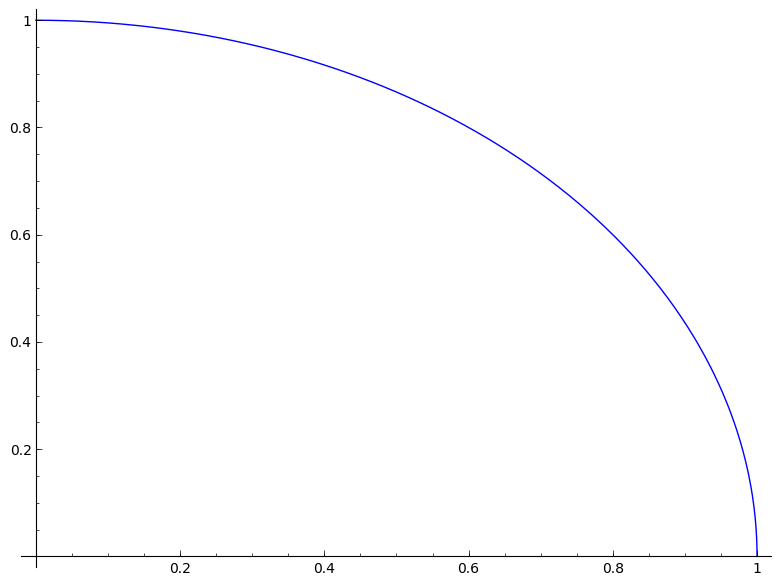
\includegraphics[scale=.25]{plot.png}\end{center}
  
  \vspace{4in}
\end{thm}

\end{document}
